\documentclass[a4paper,11pt]{exam}
	\usepackage{graphicx}
	\usepackage[utf8]{inputenc}
	\usepackage[T1]{fontenc}
	\usepackage{listings}
	\usepackage{color}
	\usepackage{amsmath}
	\usepackage{enumerate}
	\usepackage{caption}
	\usepackage{verbatim}
	\usepackage{subcaption}
	\usepackage{tikz}
	\usepackage{braket}
	\usepackage{graphics}
	\usepackage{txfonts}
	\usepackage{listings}
	\definecolor{dkgreen}{rgb}{0,0.5,0}
	\definecolor{gray}{rgb}{0.5,0.5,0.5}
	\definecolor{mauve}{rgb}{0.58,0,0.82}

	\lstset{frame=tb,
	  language=Python,
	  aboveskip=3mm,
	  belowskip=3mm,
	  showstringspaces=false,
	  columns=flexible,
	  basicstyle={\small\ttfamily},
	  numbers=none,
	  numberstyle=\tiny\color{gray},
	  keywordstyle=\color{blue},
	  commentstyle=\color{dkgreen},
	  stringstyle=\color{mauve},
	  breaklines=true,
	  breakatwhitespace=true
	  tabsize=3
	  }
	

\begin{document}
\begingroup
	  \bf \Large Mecânica Clássica II\\
	  \indent \normalsize André Del Bianco Giuffrida
	\endgroup
	\\ \quad
	\\
	\large{Fetter - Exercício \emph{4.1}}
	\\
	\\
	A thin hoop of radius $R$ and mass $M$ oscillates in its own plane with one point of the hoop fixed. Attached to the hoop is a point mass $M$
constrained to move without friction along the hoop. The system is in a uniform gravitational field $g$. Consider only small oscillations.\\

	\indent (a) Show that the normal-mode frequencies are \[\omega_1 = \frac{1}{2}\sqrt{\frac{2g}{R}}  \quad \text{and} \quad \omega_2 = \sqrt{\frac{2g}{R}}\]
	\indent (b) Find the normal-mode eigenvectors. Sketch the motion.\\
	\indent (c) Construct the modal matrix.\\
	\indent (d) Find the normal coordinates and show that they diagonalize the lagrangian.
	\\
	\normalsize
	\begin{figure}[!h]
	\centering
	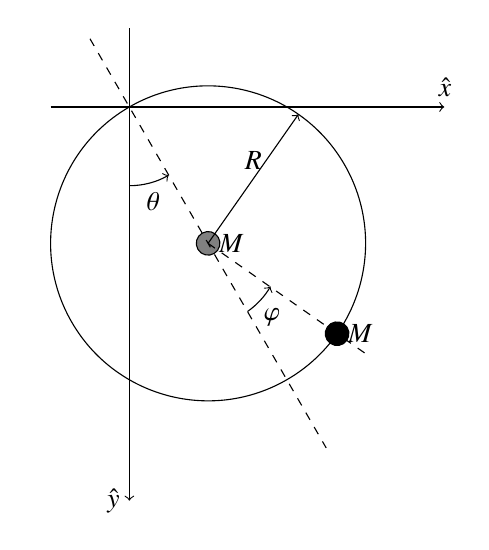
\begin{tikzpicture}
		\draw[->] (-1,0) -- (4,0) node[above] {$\hat{x}$};%x-axis
		\draw[->] (0,1) -- (0,-5) node[left] {$\hat{y}$};%y-axis
		\draw[->,rotate=-60] ([shift=(30:1cm)]0,-1) arc (-30:0:1);
		\node at (0.3,-1.2) {$\theta$};
		\begin{scope}[shift={( 1,-1.732 )},rotate=30]
			\draw[fill=gray] (0,0) circle (0.15)node[right] {$M$};
			\draw[dashed] (0,3) -- (0,-3);
			\begin{scope}[rotate=25]
				\draw[->,rotate=-85] ([shift=(30:1cm)]0,-1) arc (-25:0:1) ;
				\draw[dashed] (0,0) -- (0,-2.5);
				\node at (-0.3,-1.2) {$\varphi$};
				\draw[fill=black] (0,-2) circle (0.15) node[right] {$M$};
				\draw[->] (0,0) -- (2,0) node[midway,above] {$R$};
			\end{scope}
			\draw (0,0) circle (2);
		\end{scope}
	\end{tikzpicture}
	\end{figure}
	Podemos partir da lagrangiana usando o centro de massa para o aro.
	\[\mathcal{L} = \frac{1}{2} 2MR^2\dot\theta^2 + \frac{1}{2} MR^2((-\sin(\theta)\dot\theta-\sin(\phi)\dot\phi)^2 + (\cos(\theta)\dot\theta+\cos(\phi)\dot\phi)^2) + V(\theta,\phi)\]
	
	\[\mathcal{L} = \frac{1}{2} 2MR^2\dot\theta^2 + \frac{1}{2} MR^2(2\dot\theta^2+2\dot\phi^2 +2\dot\theta\dot\phi (\sin(\theta)\sin(\phi) +\cos(\theta)\cos(\phi)) + V(\theta,\phi)\]
	
	\[\mathcal{L} = \frac{1}{2} 2MR^2\dot\theta^2 + \frac{1}{2} MR^2(2\dot\theta^2+2\dot\phi^2 +2\dot\theta\dot\phi \cos(\theta - \phi)) + V(\theta,\phi)\]
	\[V(\theta,\phi) = MgR\cos(\theta) + MgR(\cos(\theta)+\cos(\phi)\]
	\[\mathcal{L} = \frac{1}{2} 2MR^2\dot\theta^2 + \frac{1}{2} MR^2(2\dot\theta^2+2\dot\phi^2 +2\dot\theta\dot\phi \cos(\theta - \phi)) + MgR(2\cos(\theta) +\cos(\phi) )\]
	Fazendo a aproximação para pequenos angulos, ou seja fazendo a lagrangeana quadratica:
	\[\cos(\alpha) = (1-\alpha^2/2) \quad \text{,} \quad \sin(\alpha) = \alpha\]
	
	\[\mathcal{L} = \frac{1}{2} 2MR^2\dot\theta^2 + \frac{1}{2} MR^2((2\dot\theta^2+2\dot\phi^2 +2\dot\theta\dot\phi ) + MgR\Bigg(2\Big(1-\frac{\theta^2}{2}\Big) +\Big(1-\frac{\phi^2}{2}\Big)\Bigg)\]
	
	\[\mathcal{L} = \frac{1}{2} 2MR^2\dot\theta^2 + \frac{1}{2} MR^2(2\dot\theta^2+2\dot\phi^2 +2\dot\theta\dot\phi ) - MgR\Bigg(\theta^2 +\frac{\phi^2}{2}\Bigg) + 3MgR\]
	
	\[\mathcal{L} = \frac{1}{2} 2MR^2\dot\theta^2 + \frac{1}{2} MR^2(2\dot\theta^2+2\dot\phi^2 +2\dot\theta\dot\phi ) - MgR\Bigg(\theta^2 +\frac{\phi^2}{2}\Bigg) + V_0\]
	
	
	\[\mathcal{L} = \frac{1}{2} MR^2\Bigg[4\dot\theta^2+2\dot\phi^2 +2\dot\theta\dot\phi \Bigg] - MgR\Bigg(\theta^2 +\frac{\phi^2}{2}\Bigg) + V_0\]
	
	
	Podemos escrever na forma geral, onde $R\theta = \eta_1$ e a derivada $R^2\dot\theta^2 = \dot\eta_1^2$ analogamente, $R\phi = \eta_2$ e a derivada $R^2\dot\phi^2 = \dot\eta_2^2$
	
	\[\mathcal{L} = \frac{1}{2} M\Bigg[4\dot\eta_1^2+2\dot\eta_2^2 +2\dot\eta_1\dot\eta_2 \Bigg] - \frac{Mg}{R}\Bigg(\eta_1^2 +\frac{\eta_2^2}{2}\Bigg) + V_0\]
	Usando a notação de \emph{bra-kets} $\bra{\eta}$,$\ket{\eta}$
	\[\mathcal{L} = \frac{1}{2}\Bra{\dot\eta}\, \mathcal{M} \,\Ket{\dot\eta} - \frac{1}{2}\Bra{\eta}\, \mathcal{V} \,\Ket{\eta}\]
	Onde podemos encontrar as matrizes $\mathcal{M}$ e $\mathcal{V}$.
	
	\[ \mathcal{M} = M\begin{pmatrix}
		4 & 1 \\
		1 & 2
		\end{pmatrix}
		\quad
		\text{e}
		\quad
	\mathcal{V} = \frac{Mg}{R}
		\begin{pmatrix}
			1 & 0 \\
			0 & \frac{1}{2}
		\end{pmatrix}
	\]
	Desenvolvendo por Euler-Lagrange.
	\[ \mathcal{M}\ket{\,\ddot\eta \,} + \mathcal{V}\ket{\,\eta\,} = 0\]
	\[\ket{\,\eta\,} = \cos(\omega t + \phi)\ket{\,\rho\,}\]
	Chegamos a equação de Auto-Valores:
	\[ \Big( \mathcal{V} - \mathcal{M}\omega^2 \Big)\ket{\,\rho\,} = 0 \]
	Ou seja resolvendo, $\det(\mathcal{V} - \mathcal{M}\omega^2 )=0$ podemos encontrar os valores de $\omega^2$ ou seja, os Modos Normais.
	
	Assim:
	\[ \det\begin{pmatrix}
			\frac{Mg}{R}-4M\omega^2  & -M\omega^2\\
			-M\omega^2 & \frac{Mg}{2R}-2M\omega^2
		\end{pmatrix} = 0\]
	\[\Bigg(\frac{Mg}{R}-4M\omega^2\Bigg)\Bigg(\frac{Mg}{2R}-2M\omega^2\Bigg) -M^2\omega^4 = 0\]
	\[\frac{M^2g^2}{2R^2}-\frac{4M^2g\omega^2}{R} -\frac{2M^2g\omega^2}{R} + 7M^2\omega^4 = 0\]
	\[\frac{g^2}{2R}-6g\omega^2 + 7\omega^4 R = 0\]
	
\end{document}
